% document formatting
\documentclass[10pt]{article}
\usepackage[utf8]{inputenc}
\usepackage[left=1in,right=1in,top=1in,bottom=1in]{geometry}
\usepackage[T1]{fontenc}
\usepackage{xcolor}

% math symbols, etc.
\usepackage{amsmath, amsfonts, amssymb, amsthm}

% lists
\usepackage{enumerate}

% images
\usepackage{graphicx} % for images

% code blocks
\usepackage{minted, listings} 

% verbatim greek
\usepackage{alphabeta}

\graphicspath{{./assets/images}}

\newcommand{\solution}{\textbf{Solution:}} 
\newcommand{\example}{\textbf{Example: }}
\newcommand{\R}{\mathbb{R}}

\title{BIOMATH 208 Week 1}

\author{Aidan Jan}
\date{\today}

\begin{document}
\maketitle
\section*{Overview}
\begin{enumerate}
    \item Representing and visualizing imaging data
    \begin{itemize}
        \item Pixels, vectors, etc.
    \end{itemize}
    \item Multilinear Algebra
    \begin{itemize}
        \item Linear algebra with stuff added on top
        \item Two types of square matrices
    \end{itemize}
    \item Curves and surfaces
    \begin{itemize}
        \item Comparing curves and surfaces using multilinear algebra
    \end{itemize}
    \item Manifolds
    \item Transformation Groups
    \begin{itemize}
        \item Understanding rotation, linear transformations
    \end{itemize}
    \item Tangent spaces
    \item Optimization and image registration
    \begin{itemize}
        \item Aligning multiple images of the same object
    \end{itemize}
    \item Metric manifolds
    \begin{itemize}
        \item Finding distance between two rotation matrices, ellipsoids, probabilities, etc.
        \item Using distances to compute averages, make predictions, etc.
    \end{itemize}
    \item Averaging filtering and regression
\end{enumerate}

\section*{Representing images}
\begin{itemize}
    \item Definition (images): We generally consider images as functions from some set $X \subseteq \mathbb{R}^d$, to some other set, $S$.
    \begin{itemize}
        \item $X$ describes space; usually, $d = 2$ or $d = 3$, depending on the dimension of the image.
    \end{itemize}
    \item What this means:
    \begin{itemize}
        \item Let $X$ represent a picture, some 2D set of pixels in this example.  Let $x \subset X$, where $x$ is a pixel in the picture.
        \item We can define the image, $I$, as a function, such that $X \::\: X \rightarrow S$, where $S$ is a pixel value.
        \begin{itemize}
            \item $S \in \R$ if the image is grayscale, and $S \in R^3$ if the image is colored.
        \end{itemize}
    \end{itemize}
\end{itemize}

\subsubsection*{Example 1}
\begin{center}
    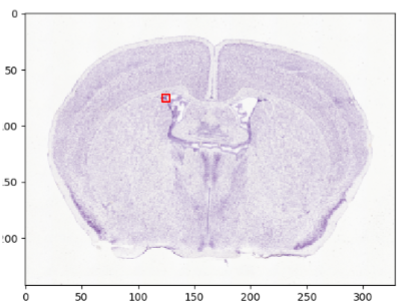
\includegraphics[scale=1]{W1_1.png}
\end{center}
\begin{itemize}
    \item Above is a microscopy image of a Nissl stained mouse brain.
    \item Here, $d = 2$ with $X$ some rectangle, and $S = [0, 1]^3$ containing $3$ RGB values, each value between 0 and 1.
\end{itemize}

\subsubsection*{Example 2}
\begin{center}
    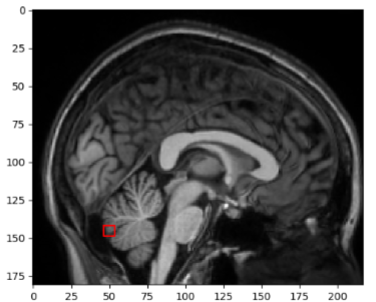
\includegraphics[scale=1]{W1_2.png}
\end{center}
\begin{itemize}
    \item Above is a part of a human brain MRI.  The set $X$ is shown on the axes.
    \item Here, $d = 3$, since this is a 3D image.  $S = \R$ since it is grayscale, therefore only one value.
    \begin{itemize}
        \item The $S$ value is a value between $[0, 1]$ representing the brightness of the pixel.
    \end{itemize}
\end{itemize}

\subsubsection*{Example 3 - Label Images}
\begin{center}
    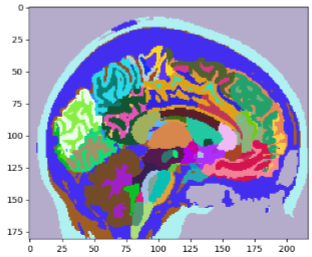
\includegraphics[scale=1]{W1_3.png}
\end{center}
\begin{itemize}
    \item Here, $d = 3$ with $X$ some rectangular prism, and $S = \mathbb{N}$ containing 1 integer, \texttt{id}.  Each \texttt{id} represents some particular type of structure.  
    \item Part of a labeled brain image is shown.  Integers are shown as colors, and the set $X$ is shown on the axes for one slice of the 3D volume.
\end{itemize}

\subsection*{Discrete Images}
\begin{itemize}
    \item Treating images as functions is nice, because they have basically infinite resolution.  (You can plug in any coordinate value and receive the corresponding values.)
    \item However, we can't store the functions in a computer.  As a result, we usually work with \textbf{discrete images}.
    \item In this case, images are $d$-dimensional arrays, storing values in $S$.
    \begin{itemize}
        \item Geometry is stored with pixel size $\Delta \in \R^d$, and origin $O \in \R^d$.
        \item Square brackets are used to index starting from 0. \texttt{img[0, 0]} would represent the top left corner.
        \item In 3D, we would use rows, columns, and slices.
        \item We may also specify the location of the origin, $O$, to scale in real life.  Origin is \texttt{img[0, 0]}, but may be assigned some real world location, for example, [10ft, 20ft].  $\Delta$ is the pixel size, and therefore the physical location for any pixel can be calculated.  (Real location of pixel \texttt{img[i,j]} would be $O + \Delta \cdot {i \choose j}$).
    \end{itemize}
\end{itemize}

\subsection*{Grayscale images}
\begin{center}
    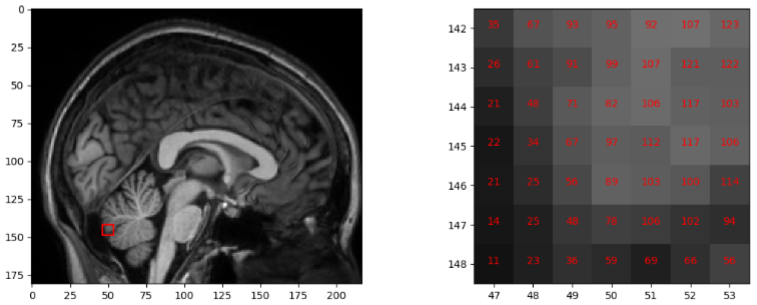
\includegraphics[scale=1]{W1_4.png}
\end{center}
\begin{itemize}
    \item Here we see a sagittal view of a brain MR image, and a zoom in showing pixel values.
    \item Here, the origin is (0, 0), and the spacing is (1, 1) (in mm).
\end{itemize}

\subsection*{Color Histology}
\begin{center}
    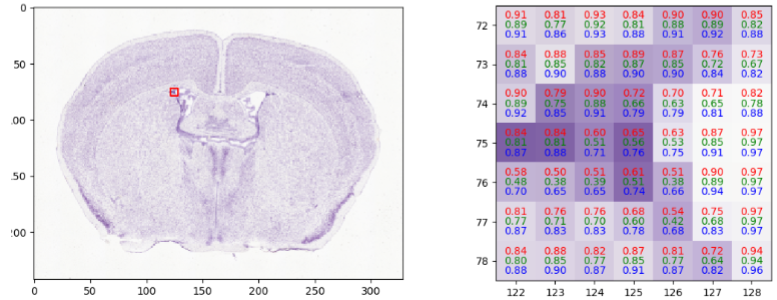
\includegraphics[scale=1]{W1_5.png}
\end{center}
\begin{itemize}
    \item Here we see an image, and a zoom in showing pixel values as RGB triples.
    \item Here the origin is (0, 0), and the spacing is (58.8, 58.8) (in microns).
\end{itemize}

\section*{Interpolation}
Interpolation links images as functions to images as discrete arrays.  If $S$ is a vector space, then we can specify an interpolation kernel $h$ and write
\[I(x) = \sum_{i, j, k} I[i, j, k] h(x - x[i, j, k])\]
where $x[i, j, k] = O + \text{diag}(\Delta)\begin{pmatrix} i \\ j \\ k \end{pmatrix}$, the coordinate of the $i, j, k$-th pixel.
\begin{itemize}
    \item $I(x)$ is the image function, and $I[i, j, k]$ is the array of pixels.  $h$ is often a function that is close to 1 near the origin and decays down to zero as you get far away.  
    \begin{itemize}
        \item $h()$ is also known as a point-spread function (psf), or an impulse response function.
    \end{itemize}
    \item What the function basically does is that it multiplies the pixel value by the impulse response function at that real-world location.
    \item We are convolving the kernels with the discrete pixel dataset.  Triangle kernel gives linear interpolation, and rectangle kernel gives nearest neighbor interpolation.
\end{itemize}
\begin{center}
    \includegraphics*[scale=1]{W1_6.png}
    \includegraphics*[scale=1]{W1_7.png}
\end{center}
\begin{itemize}
    \item The image on the left is a brain interpolated (convolved) using the rectangle kernel
    \item The middle image is one interpolated with the triangle kernel
    \item The right image is a brain interpolated with a piecewise cubic function (aka. third degree spline).
\end{itemize}
Importantly, the range of values the function takes is the same as the values.  Since the kernel function is always between values 0-1, the minimum value of the interpolated image is 0, and the maximum is the highest original pixel value.

\subsection*{2D grayscale images}
\begin{itemize}
    \item To display images, intensity values at each pixel need to be mapped to a brightness value on the screen (a number between 0 and 1)
    \item A piecewise linear function is used to do this, by selecting a lower value for black, and an upper value for white.
    \item A histogram of pixel values can be used to choose these parameters.
\end{itemize}
\begin{center}
    \includegraphics*[scale=1]{W1_8.png}
\end{center}
\begin{itemize}
    \item The histogram is one that shows pixel values.  The center should be set at the highest peak of the contrast map, e.g., setting brightness and contrast.
    \item The brightness value is essentially "which pixel value should be mapped to black", and contrast is the "difference between white pixel and black pixel" or, "what pixel value is white relative to black".
    \item The above image sets black to 0 HU, and white to 80 HU.  Anything below the range is black, anything above is white.
\end{itemize}
\end{document}
